%!TeX spellcheck = <engl>
%
% File: chap01.tex
% Author: Victor F. Brena-Medina
% Description: Introduction chapter where the biology goes.
%
\let\textcircled=\pgftextcircled
\chapter{Conclusion and Future Work}
\label{chap:fw}

This project developed two novel methods to detect and characterise contexts from images and point clouds respectively. The methods have been tested on the KITTI dataset and image context detection has proved to be quite accurate as compared to point cloud context detection.
I have shown that cutting edge multimodal and LiDAR only methods perform differently in urban and non-urban environments with multimodal methods performing much better in urban environments and LiDAR only performing close to multimodal methods in non-urban contexts. Furthermore I was able to establish that it is possible to run a multimodal method(AVOD) in urban contexts and a LiDAR only model(VoxelNet) simultaneously on a single GPU optimally. 
This opens up the possibility of a pipeline model whereby depending on the context, it may be possible to switch to a different model without being affected. Figure \ref{fig:pipeline} illustrates a prototype of such a system. 
\begin{figure}[h] %Pipeline
	\centering 
	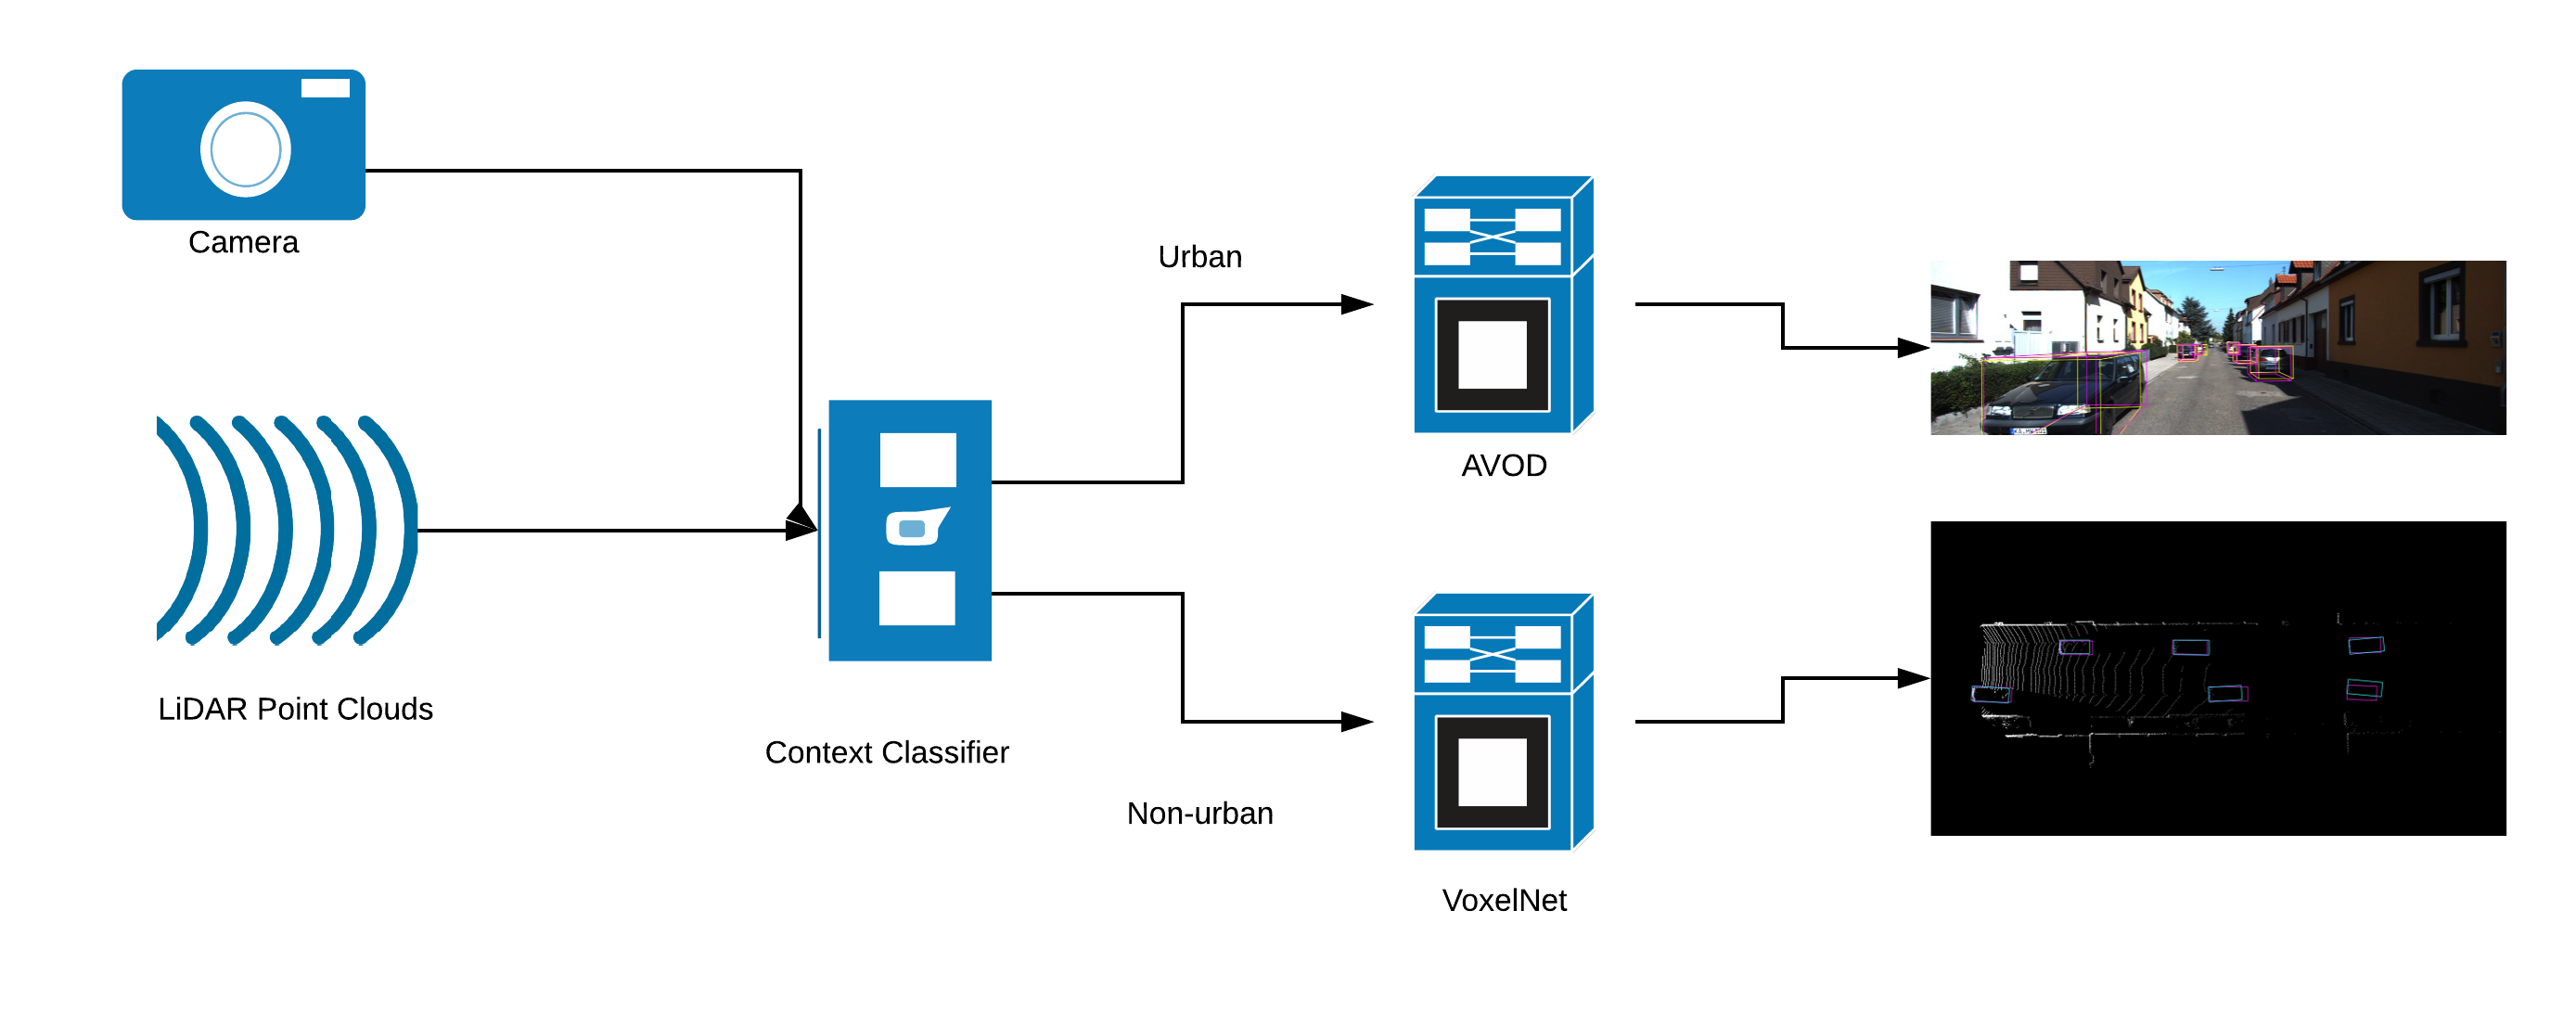
\includegraphics[width=\linewidth]{images/pipeline}	
	\caption{Context-Dependent Model Pipeline Prototype}
	\label{fig:pipeline}

\end{figure}
The GPU metrics and graph statistics were able to provide an insight into the correlation between the temperature generation and FLOPS as well as between the number of parameters and memory usage whereby higher FLOPs resulted in higher temperatures and similarly, higher parameters resulted in higher memory usage. 

The downsides of LiDAR only methods in terms of generalising to different LiDAR sensors was also established whereby the frequency in terms of points returned per second affected the point cloud density and consequently VoxelNet did not produce any predictions when run through the SIL dataset with low point cloud density. This highlighted the need to either standardise the use of specific sensors with high frequency or to develop sensor-agnostic object detection models that can generalise to different sensors and datasets. Alternatively, depth filling methods can be utilised to increase the denseness of these point clouds before being used as input\cite{depth}. 

A final contribution was to make publicly available the SIL dataset with annotated samples that can be used in developing new object detection models and testing existing ones to improve their generalisation. 

\section{Future Work}
Despite being able to fulfill the objectives set out, this project can be further improved in future iterations. 
Firstly, the process of context detection can be implemented using deep learning methods to enable automatic feature extraction instead of using manual feature extraction using histograms and descriptors. This could be similar to the feature extractor layers in AVOD that are able to extract features automatically from images and point clouds as well. In addition, a more accurate point cloud context detector can be developed to use the feature maps generated by these feature extractors that have high representation and resolution. Furthermore, it is possible to extend the implementation into an end to end model that can be trained all at once. 

Another avenue for future work could be exploring the use different accelerators other than the GPUs. \cite{lin2018architectural} investigated the use of ASIC, FPGAs and GPU for different tasks such as detection, tracking and localisation and established that using ASICs and FPGA could restrain the driving range reduction to around 5\%. This could be further improved by using models with lightweight architectures with low memory and computational power requirements. A recently published model that tries to achieve this is \cite{wang2018pointseg}. 

\section{Personal Reflection}

This project greatly helped me understand various perspectives on the development of AVs. Beginning from the technical, legal and even economic aspects that form the driving force for different design choices. This project evolved from simply trying to replicate the VoxelNet model that was not publicly released to later on realising a gap in the assessment of object detection models in different contexts and went further on to realising the impact of different LiDAR sensors on the performance of these models. This process helped me understand more about how the development of such systems tends to be quite complex and involves the collaboration of different disciplines to better understand how they can be fully integrated.

In terms of programming, the graph model abstraction of the Tensorflow framework presented a steep learning curve for me as I was used to imperative programming frameworks. As a result, debugging was initially quite difficult but with time, I was able to understand how to modify the computational graph. This was especially the case while implementing the focal loss function that resulted in "inf and nan" errors. Another time consuming element was hyper parameter tuning for the networks. Most models that were released in public did not include the best parameters for training these networks, as such a lot of time was spent in finding the best parameters\footnote{See appendix {\ref{chap:res}}}. CometML greatly helped in tracking the parameters that were the best performing and provided a facility to automatically create a GitHub pull request for them. 	

 In addition, working with point clouds tended to be quite difficult as there are not many Python libraries that can manipulate point clouds and those that are available do not support as many features. As a result, a lot of time was spent in researching different methods to manipulate the point clouds for the task of context and object detection. This resulted in using a lot of boiler-plate code using different libraries. If there was enough time, this could've been improved by compiling these functions into one library that could provide these functions in a simpler object oriented method. 
 